% Chapter 1

\chapter{Introduction} % Main chapter title
\addchaptertocentry{Introduction} 
\label{Introduction} % For referencing the chapter elsewhere, use \ref{Chapter1} 

%----------------------------------------------------------------------------------------

% Define some commands to keep the formatting separated from the content 
\newcommand{\keyword}[1]{\textbf{#1}}
\newcommand{\tabhead}[1]{\textbf{#1}}
\newcommand{\code}[1]{\texttt{#1}}
\newcommand{\file}[1]{\texttt{\bfseries#1}}
\newcommand{\option}[1]{\texttt{\itshape#1}}

%----------------------------------------------------------------------------------------

\section{Vision naturelle}
>> Rôle de la vision\\
Tous  les êtres vivants utilisent la vision à un degré ou à un autre, et pour de nombreuses espèces -y compris la notre- elle est même la modalité perceptive principale. Chez nous, cette dominance de la vision transcende la notion de modalité perceptive et s'ancre dans notre culture, que ce soit au travers des arts ou du language (qui n'a jamais dit un jour ''Ah, je vois!'') ainsi que dans la construction de nos relations sociales, nous permettant de capter ou d'exprimer émotions et intentions.

>> Structure générale d'une rétine (cônes/bâtonnets + fovéa/rétine périphérique)\\
Chez les vertébrés la vision débute à la surface de la rétine, où les cellules photovoltaïques (cônes et bâtonnets) réalisent la transduction des signaux lumineux qui les atteignent en signaux électriques, transmissibles à la suite du réseau nerveux.\\
Les cônes et les bâtonnets sont différenciées par un certain nombre de caractéristiques, notamment leur sensibilité aux longueurs d'ondes lumineuses et leur distribution au sein de la rétine. Ces différences permettent à notre rétine de rester fonctionnelle dans de nombreuses situations, y compris lorsque la luminance est très faible (le seuil absolu de la rétine humaine correspondant à 70 photons) et permet donc à la modalité visuelle de nous fournir des informations pertinentes dans un large champs de contextes.\\
Les bâtonnets sont plus nombreux que les cônes et sensibles à des variations de luminance plus fines. Ils sont majoritairement responsables de notre vision scotopique (dans des conditions de faible luminance, tel que la nuit) et sont des acteurs majeurs de la vision périphérique.\\
Le champs visuel peut être divisé en vision centrale et vision périphérique. La vision centrale (environ \SI{2}{\degree}) est soutenue par la région rétinienne appelée fovea, comprenant uniquement des cônes. On y observe l'acuité visuelle la plus importante (elle représente seulement 1\% de la rétine mais plus de 50\% du cortex visuel est attribué au traitement de son activité). Cette acuité visuelle diminue avec l'excentricité par rapport à la fovéa(\cite{Werner2014}).

>> Notion de saccades oculaires/Vision d'une cible en périphérie\\
Lors de l'exploration de son environnement visuel, un agent va en conséquence réaliser des saccades oculaires : mouvements brefs (20-60\si{\milli\second}) des globes oculaires (réalisés grâce aux muscles oculomoteurs les encadrant) afin de placer l'image d'une cible (ou sa position prédite dans l'espace) au niveau de la fovéa, permettant ainsi de traiter les informations en provenant avec la plus grande préçision possible.

>> Cellules parvo/magno -> rôle de la voie magno\\
L'activité rétinienne est transmise le long des voies nerveuses visuelles jusqu'au cortex visuel, où sera réalisé la majorité du traitement des informatiques qu'elle supporte. \\
Entre la rétine et le cortex existe un certain nombre d'étapes, mais tout au long de ces voies, la distribution rétinienne de l'information  (la rétinotopie) est conservée. 

\begin{figure}[th]
\centering
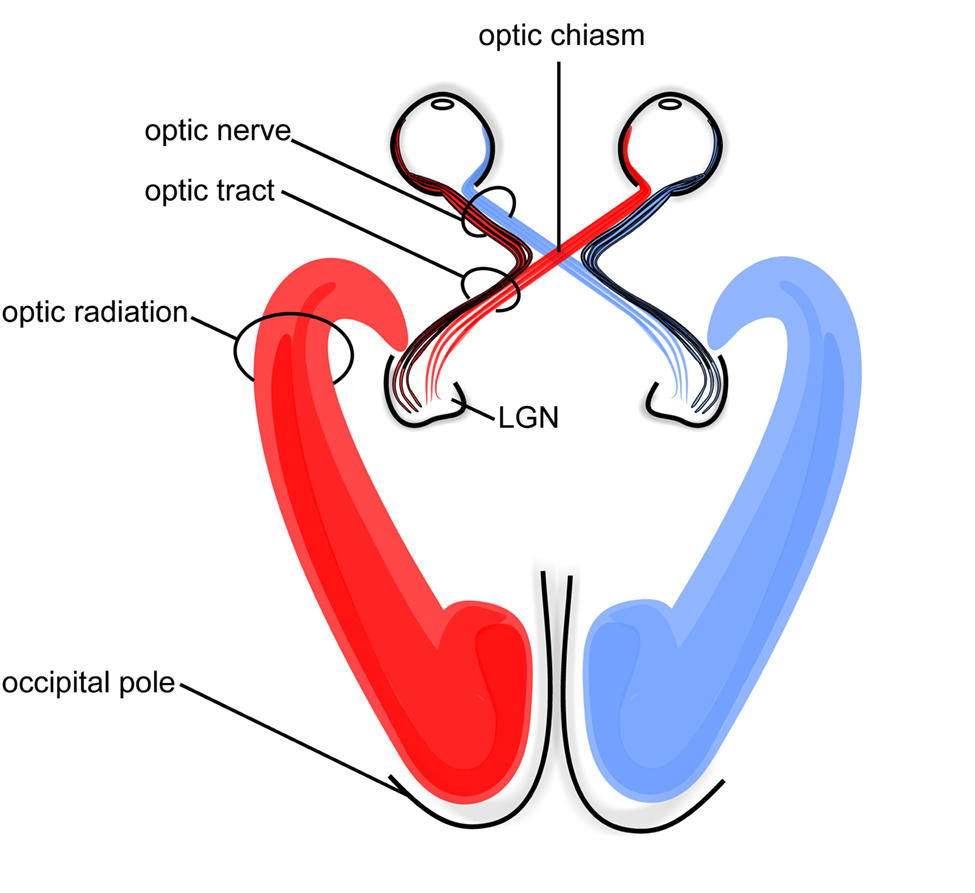
\includegraphics{Figures/visual_system}
\decoRule %puts an aesthetic horizontal line below the image
\caption[Figure]{Schéma des voies visuelles humaines, de la rétine jusqu'au cortex visuel primaire (adapté de Hofer S. et al., 2010 via Wikimedia Commons [CC BY 3.0]}
\label{fig:visual_system}
\end{figure}

Dans leurs travaux de 1962 et 1977, Hubel et Wiesel émettent l'hypohèse des courants visuels, qui définit trois grandes voies visuelles : magnocellulaire (M), parvocellulaire (P) et koniocellulaire (K). Chacune supporte le transport d'informations visuelles présentant des caractèristiques distinctes (\cite{Werner2014}).

>> Voie dorsale (voie du "où/where"), rôle dans la localisation de cible\\

%----------------------------------------------------------------------------------------

\section{Vision artificielle}
>> Motivations

\begin{equation}
E = mc^{2}
\label{eqn:Einstein}
\end{equation}

If you don't want a particular equation numbered, use the unnumbered form:
\begin{verbatim}
\[ a^{2}=4 \]
\end{verbatim}
